\section{Introduction}
\label{sec:introduction}

\PARstart{E}{ight} PMUs observe only a small part of a 39-bus network,
yet an operator needs to know whether a disturbance occurred, which
physical mechanism caused it, and where it began. An unmeasured bus can
change several remote PMU signals, while different sources can produce
similar measured responses. The problem is therefore both electrical
and statistical: reconstruct the response allowed by the network, then
compare its possible causes under uncertain state, severity and noise.

Our starting point is a feature-based hackathon system. Voltage, current,
frequency and spatial/temporal descriptors supported an ExtraTrees
detector, classifier and localizer. We retain that route and its results.
The complementary route asks an explicit counterfactual question: if this
source had changed at a candidate past time, what would all eight PMUs
have measured up to now? Physical equations provide the candidate path;
conditional Bayesian evidence accounts for unknown severity and competing
histories. After restoration, those histories must still explain the
remaining machine motion.

\begin{figure*}[t]\centering
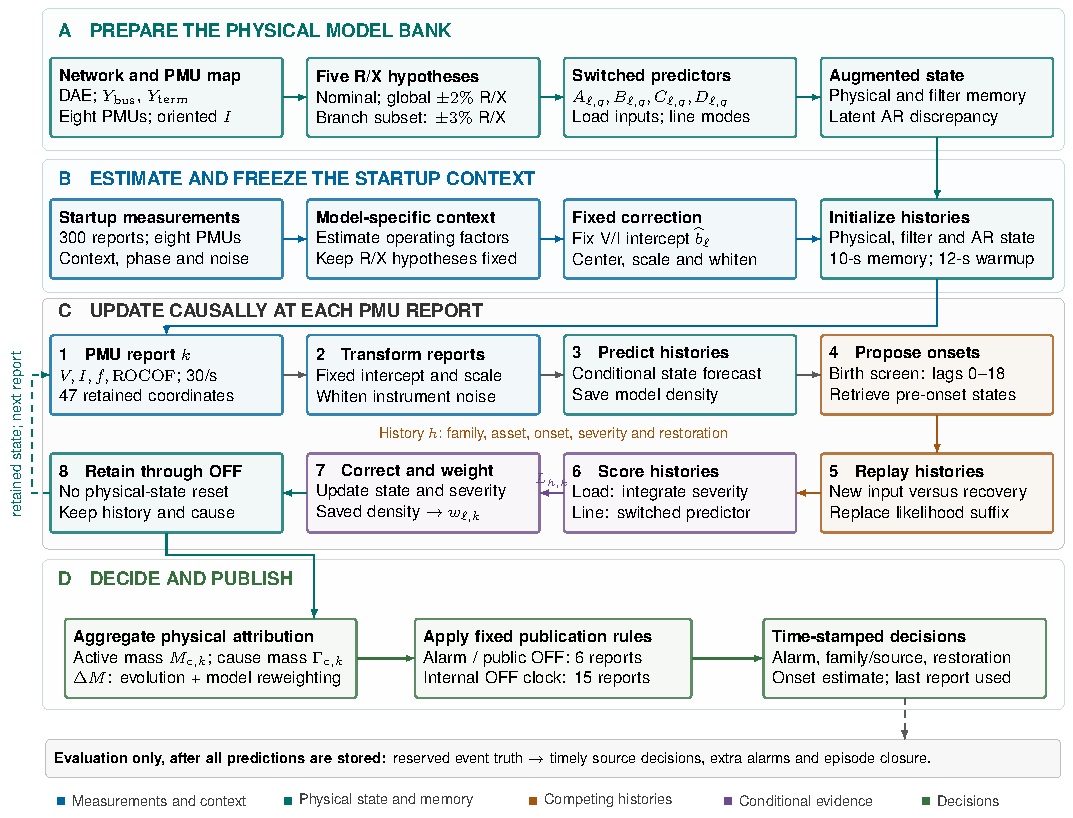
\includegraphics[width=.98\textwidth]{figures/generated/narrative_architecture.pdf}
\caption{Implemented physical inference in four stages. (A) Construct switched network and PMU predictors. (B) Estimate the startup context and fix its observation correction. (C) Compare new intervention histories with retained recovery at each report, using stored pre-onset states. (D) Aggregate attribution and publish qualified alarm, source and restoration decisions. The public six-report rules and the internal 15-report OFF clock are distinct; their support conditions are specified in Section~\ref{sec:narrative-method}. Dashed feedback retains state for the next report. Reserved truth enters only the later evaluation.}
\label{fig:joint-architecture}\end{figure*}

Physical restoration does not erase machine motion. A flat reference can
mislabel its remaining oscillation as a second event; suppressing all alarms
during recovery can hide an actual second event. A corrected voltage offset
also need not correct the response to a later input.

DAE estimators recover unmeasured electrical states
\cite{katanic2024recursive}; outage detectors compare physical hypotheses
\cite{chen2016quickest,rovatsos2017outage}; and simulated trajectories
support sparse-PMU fault diagnosis \cite{warner2023highfidelity}. These
ingredients are established. Our question is whether a continuing recovery
should explain a new PMU change or yield to a later intervention hypothesis.

The contribution is a specified causal attribution procedure and an
empirical account of where physical structure helps and fails. Three
results connect the earlier components to the complete comparison:
\begin{enumerate}
\item Network-conditioned state reconstruction, physical feature ablations
and mixed-source sensitivity experiments quantify three ways of extracting
information from sparse PMUs. Their contracts and limits are reported
separately; they are not presented as one already validated joint filter.
\item The continuous procedure compares new interventions with retained
recovery histories, integrates local load severity, and separates active
mass $M$ from originating-cause mass $\Gamma$. Its $\Delta M$ records the
changing attribution. The predictor and Bayesian history calculation,
rather than the array's shape, carry the physical information.
\item A direct historical transfer of the submitted system and a new
same-stream comparison with causal ExtraTrees distinguish feature failure,
source attribution and alarm cost. The latter also compares a published
outage detector on its eligible persistent-line task.
\end{enumerate}
The complete physical bank attributes
\ReaderPhysicalLoad{}/\ReaderFamilyTotal{} load realizations before OFF
versus \ReaderETLoad{}/\ReaderFamilyTotal{} for the causal ExtraTrees
reference. Under out-of-bank R/X it raises \ReaderPhysicalOutsideExtras{}
versus \ReaderETOutsideExtras{} unmatched alarms. Thus the supported gain
is timely load attribution with a larger alarm burden, not uniformly
better diagnosis. Neither the isolated benefit of recovery memory nor an
end-to-end accuracy gain caused specifically by tensor/Bayes components
has been measured.

The test uses nine candidate load buses and nine lines in a fixed IEEE-39
simulation. It does not establish an all-family hackathon score, calibrated
event probabilities or real-time deployment.
